\documentclass[12pt,a4paper,titlepage,twoside,openright]{article}
\usepackage[english]{babel}
\usepackage{ucs} 
\usepackage[utf8x]{inputenc}
\usepackage[usenames,dvipsnames]{xcolor}
\usepackage{tikz,pgfplots}
\usepackage{tkz-tab}
\usepackage{caption}
\usepackage{latexsym}
\usepackage{amssymb}
\usepackage{amsmath}
\usepackage{subcaption} 

\begin{document}

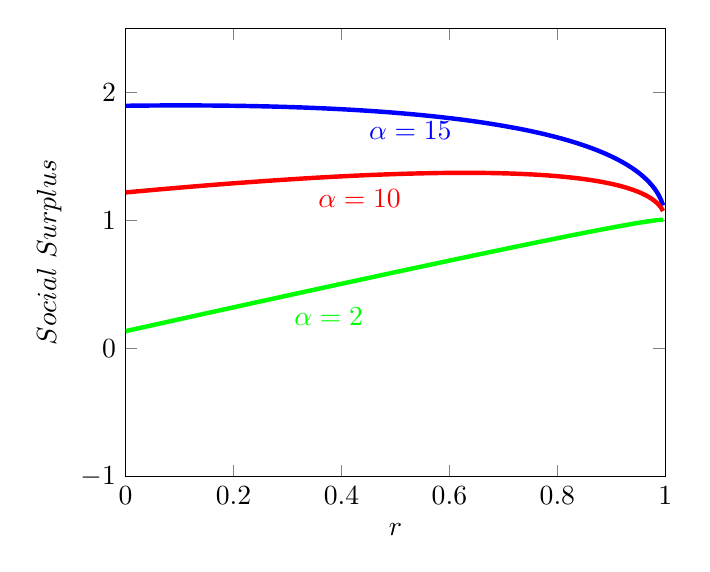
\begin{tikzpicture}
\begin{axis}[ 
xlabel=$r$,
ylabel={$Social~Surplus$}, xmin=0,xmax=1,ymin=-1,ymax=2.5 ]

\addplot[domain=0:1,samples=250, ultra thick, blue ]{ 
15*sqrt(1-x) 
-exp(ln((15-1)*sqrt(1-x))-2) 
-x(1+ln((15-1)*sqrt(1-x)-2)-ln((15-1)*sqrt(1-x))*(1-sqrt(1-x)))
+1
-2(exp(ln((15-1)*sqrt(1-x))-2)+x)}node [pos=0.3, below right] {$\alpha = 15$};
\addplot[domain=0:1,samples=250, ultra thick, red ]{ 
10*sqrt(1-x) 
-exp(ln((10-1)*sqrt(1-x))-2) 
-x(1+ln((10-1)*sqrt(1-x)-2)-ln((10-1)*sqrt(1-x))*(1-sqrt(1-x)))
+1
-2(exp(ln((10-1)*sqrt(1-x))-2)+x)} node [pos=0.3, below right] {$\alpha=10$}; 
\addplot[domain=0:1,samples=250, ultra thick, green ]{ 
2*sqrt(1-x) 
- exp(ln((2-1)*sqrt(1-x))-2) 
-x(1+ln((2-1)*sqrt(1-x)-2)-ln((2-1)*sqrt(1-x))*(1-sqrt(1-x)))
+1
-2(exp(ln((2-1)*sqrt(1-x))-2)+x)}node [pos=0.3, below right] {$\alpha=2$}; 
\end{axis}
\end{tikzpicture}

\end{document}